%% Beginning of file 'sample631.tex'
%%
%% Modified 2022 May  
%%
%% This is a sample manuscript marked up using the
%% AASTeX v6.31 LaTeX 2e macros.
%%
%% AASTeX is now based on Alexey Vikhlinin's emulateapj.cls 
%% (Copyright 2000-2015).  See the classfile for details.

%% AASTeX requires revtex4-1.cls and other external packages such as
%% latexsym, graphicx, amssymb, longtable, and epsf.  Note that as of 
%% Oct 2020, APS now uses revtex4.2e for its journals but remember that 
%% AASTeX v6+ still uses v4.1. All of these external packages should 
%% already be present in the modern TeX distributions but not always.
%% For example, revtex4.1 seems to be missing in the linux version of
%% TexLive 2020. One should be able to get all packages from www.ctan.org.
%% In particular, revtex v4.1 can be found at 
%% https://www.ctan.org/pkg/revtex4-1.

%% The first piece of markup in an AASTeX v6.x document is the \documentclass
%% command. LaTeX will ignore any data that comes before this command. The 
%% documentclass can take an optional argument to modify the output style.
%% The command below calls the preprint style which will produce a tightly 
%% typeset, one-column, single-spaced document.  It is the default and thus
%% does not need to be explicitly stated.
%%
%% using aastex version 6.3
\documentclass[twocolumn]{aastex631}

\usepackage{verbatim}
\usepackage{amsmath}
\usepackage{multirow}
\usepackage{relsize}


\usepackage{amssymb}
\usepackage{float}
\usepackage{hyperref}

\graphicspath{{figs/}}

\newcommand{\bb}[1]{{\textcolor{blue}{[bb: #1]}}}
\newcommand{\sigs}{\sigma_s}
\newcommand{\dv}[1]{{\color{red}dv: #1}}
\newcommand{\kpo}[1]{{\color{red}kpo: #1}}
\newcommand{\mm}[1]{{\textcolor{purple}{[mm: #1]}}}
%%%%%%%%%%%%%%%%%%%%%%%%%%%%%%%%%%%%%%%%%%%%%%%%%%%%%%%%%%%%%%%%%%%%%%%%%%%%%%%%

%\submitjournal{ApJ}

\shorttitle{Energy Budgets of Galaxy Merger}
\shortauthors{Motka et al.}

%%%%%%%%%%%%%%%%%%%%%%%%%%%%%%%%%%%%%%%%%%%%%%%%%%%%%%%%%%%%%%%%%%%%%%%%%%%%%%%%


%% The default is a single spaced, 10 point font, single spaced article.
%% There are 5 other style options available via an optional argument. They
%% can be invoked like this:
%%
%% \documentclass[arguments]{aastex631}
%% 
%% where the layout options are:
%%
%%  twocolumn   : two text columns, 10 point font, single spaced article.
%%                This is the most compact and represent the final published
%%                derived PDF copy of the accepted manuscript from the publisher
%%  manuscript  : one text column, 12 point font, double spaced article.
%%  preprint    : one text column, 12 point font, single spaced article.  
%%  preprint2   : two text columns, 12 point font, single spaced article.
%%  modern      : a stylish, single text column, 12 point font, article with
%% 		  wider left and right margins. This uses the Daniel
%% 		  Foreman-Mackey and David Hogg design.
%%  RNAAS       : Supresses an abstract. Originally for RNAAS manuscripts 
%%                but now that abstracts are required this is obsolete for
%%                AAS Journals. Authors might need it for other reasons. DO NOT
%%                use \begin{abstract} and \end{abstract} with this style.
%%
%% Note that you can submit to the AAS Journals in any of these 6 styles.
%%
%% There are other optional arguments one can invoke to allow other stylistic
%% actions. The available options are:
%%
%%   astrosymb    : Loads Astrosymb font and define \astrocommands. 
%%   tighten      : Makes baselineskip slightly smaller, only works with 
%%                  the twocolumn substyle.
%%   times        : uses times font instead of the default
%%   linenumbers  : turn on lineno package.
%%   trackchanges : required to see the revision mark up and print its output
%%   longauthor   : Do not use the more compressed footnote style (default) for 
%%                  the author/collaboration/affiliations. Instead print all
%%                  affiliation information after each name. Creates a much 
%%                  longer author list but may be desirable for short 
%%                  author papers.
%% twocolappendix : make 2 column appendix.
%%   anonymous    : Do not show the authors, affiliations and acknowledgments 
%%                  for dual anonymous review.
%%
%% these can be used in any combination, e.g.
%%
%% \documentclass[twocolumn,linenumbers,trackchanges]{aastex631}
%%
%% AASTeX v6.* now includes \hyperref support. While we have built in specific
%% defaults into the classfile you can manually override them with the
%% \hypersetup command. For example,
%%
%% \hypersetup{linkcolor=red,citecolor=green,filecolor=cyan,urlcolor=magenta}
%%
%% will change the color of the internal links to red, the links to the
%% bibliography to green, the file links to cyan, and the external links to
%% magenta. Additional information on \hyperref options can be found here:
%% https://www.tug.org/applications/hyperref/manual.html#x1-40003
%%
%% Note that in v6.3 "bookmarks" has been changed to "true" in hyperref
%% to improve the accessibility of the compiled pdf file.
%%
%% If you want to create your own macros, you can do so
%% using \newcommand. Your macros should appear before
%% the \begin{document} command.
%%
\newcommand{\vdag}{(v)^\dagger}
\newcommand\aastex{AAS\TeX}
\newcommand\latex{La\TeX}

%% Reintroduced the \received and \accepted commands from AASTeX v5.2
%\received{March 1, 2021}
%\revised{April 1, 2021}
%\accepted{\today}

%% Command to document which AAS Journal the manuscript was submitted to.
%% Adds "Submitted to " the argument.
%\submitjournal{PSJ}

%% For manuscript that include authors in collaborations, AASTeX v6.31
%% builds on the \collaboration command to allow greater freedom to 
%% keep the traditional author+affiliation information but only show
%% subsets. The \collaboration command now must appear AFTER the group
%% of authors in the collaboration and it takes TWO arguments. The last
%% is still the collaboration identifier. The text given in this
%% argument is what will be shown in the manuscript. The first argument
%% is the number of author above the \collaboration command to show with
%% the collaboration text. If there are authors that are not part of any
%% collaboration the \nocollaboration command is used. This command takes
%% one argument which is also the number of authors above to show. A
%% dashed line is shown to indicate no collaboration. This example manuscript
%% shows how these commands work to display specific set of authors 
%% on the front page.
%%
%% For manuscript without any need to use \collaboration the 
%% \AuthorCollaborationLimit command from v6.2 can still be used to 
%% show a subset of authors.
%
%\AuthorCollaborationLimit=2
%
%% will only show Schwarz & Muench on the front page of the manuscript
%% (assuming the \collaboration and \nocollaboration commands are
%% commented out).
%%
%% Note that all of the author will be shown in the published article.
%% This feature is meant to be used prior to acceptance to make the
%% front end of a long author article more manageable. Please do not use
%% this functionality for manuscripts with less than 20 authors. Conversely,
%% please do use this when the number of authors exceeds 40.
%%
%% Use \allauthors at the manuscript end to show the full author list.
%% This command should only be used with \AuthorCollaborationLimit is used.

%% The following command can be used to set the latex table counters.  It
%% is needed in this document because it uses a mix of latex tabular and
%% AASTeX deluxetables.  In general it should not be needed.
%\setcounter{table}{1}

%%%%%%%%%%%%%%%%%%%%%%%%%%%%%%%%%%%%%%%%%%%%%%%%%%%%%%%%%%%%%%%%%%%%%%%%%%%%%%%%
%%
%% The following section outlines numerous optional output that
%% can be displayed in the front matter or as running meta-data.
%%
%% If you wish, you may supply running head information, although
%% this information may be modified by the editorial offices.
%\shorttitle{AASTeX v6.3.1 Sample article}
%\shortauthors{Schwarz et al.}
%%
%% You can add a light gray and diagonal water-mark to the first page 
%% with this command:
%% \watermark{text}
%% where "text", e.g. DRAFT, is the text to appear.  If the text is 
%% long you can control the water-mark size with:
%% \setwatermarkfontsize{dimension}
%% where dimension is any recognized LaTeX dimension, e.g. pt, in, etc.
%%
%%%%%%%%%%%%%%%%%%%%%%%%%%%%%%%%%%%%%%%%%%%%%%%%%%%%%%%%%%%%%%%%%%%%%%%%%%%%%%%%
%\graphicspath{{./}{figures/}}
%% This is the end of the preamble.  Indicate the beginning of the
%% manuscript itself with \begin{document}.

\begin{document}

\title{Transformation of Energy Budgets during The Formation of Major MW-M31 Merger Remnant}

%% LaTeX will automatically break titles if they run longer than
%% one line. However, you may use \\ to force a line break if
%% you desire. In v6.31 you can include a footnote in the title.

%% A significant change from earlier AASTEX versions is in the structure for 
%% calling author and affiliations. The change was necessary to implement 
%% auto-indexing of affiliations which prior was a manual process that could 
%% easily be tedious in large author manuscripts.
%%
%% The \author command is the same as before except it now takes an optional
%% argument which is the 16 digit ORCID. The syntax is:
%% \author[xxxx-xxxx-xxxx-xxxx]{Author Name}
%%
%% This will hyperlink the author name to the author's ORCID page. Note that
%% during compilation, LaTeX will do some limited checking of the format of
%% the ID to make sure it is valid. If the "orcid-ID.png" image file is 
%% present or in the LaTeX pathway, the OrcID icon will appear next to
%% the authors name.
%%
%% Use \affiliation for affiliation information. The old \affil is now aliased
%% to \affiliation. AASTeX v6.31 will automatically index these in the header.
%% When a duplicate is found its index will be the same as its previous entry.
%%
%% Note that \altaffilmark and \altaffiltext have been removed and thus 
%% can not be used to document secondary affiliations. If they are used latex
%% will issue a specific error message and quit. Please use multiple 
%% \affiliation calls for to document more than one affiliation.
%%
%% The new \altaffiliation can be used to indicate some secondary information
%% such as fellowships. This command produces a non-numeric footnote that is
%% set away from the numeric \affiliation footnotes.  NOTE that if an
%% \altaffiliation command is used it must come BEFORE the \affiliation call,
%% right after the \author command, in order to place the footnotes in
%% the proper location.
%%
%% Use \email to set provide email addresses. Each \email will appear on its
%% own line so you can put multiple email address in one \email call. A new
%% \correspondingauthor command is available in V6.31 to identify the
%% corresponding author of the manuscript. It is the author's responsibility
%% to make sure this name is also in the author list.
%%
%% While authors can be grouped inside the same \author and \affiliation
%% commands it is better to have a single author for each. This allows for
%% one to exploit all the new benefits and should make book-keeping easier.
%%
%% If done correctly the peer review system will be able to
%% automatically put the author and affiliation information from the manuscript
%% and save the corresponding author the trouble of entering it by hand.

%\correspondingauthor{August Muench}
%\email{greg.schwarz@aas.org, gus.muench@aas.org}
\correspondingauthor{Jay Motka}
\email{jaymotka@arizona.edu}

\author[0000-0001-7379-2625]{Jay Motka} 
\affiliation{Department of Astronomy and Steward Observatory, University of Arizona, Tucson, AZ 85721, USA}
\date{\today}

%% Note that the \and command from previous versions of AASTeX is now
%% depreciated in this version as it is no longer necessary. AASTeX 
%% automatically takes care of all commas and "and"s between authors names.

%% AASTeX 6.31 has the new \collaboration and \nocollaboration commands to
%% provide the collaboration status of a group of authors. These commands 
%% can be used either before or after the list of corresponding authors. The
%% argument for \collaboration is the collaboration identifier. Authors are
%% encouraged to surround collaboration identifiers with ()s. The 
%% \nocollaboration command takes no argument and exists to indicate that
%% the nearby authors are not part of surrounding collaborations.

%% Mark off the abstract in the ``abstract'' environment. 
\vspace{-1cm}
\keywords{Local Group; Galaxy Merger; Merger Remnant; Major Merger; Dark Matter Halo; Virial Equilibrium}

\section{Introduction}
\label{sec:intro}

Milky Way (MW) along with its largest neighbour the Andromeda galaxy (M31) and a collection of the satellite galaxies that orbit them makes up a group of galaxies called the Local Group. The largest of these satellite galaxies is the Triangulum galaxy (M33). According to \cite{simulation}, the MW and M31 will merge at $t = 5.86^{+1.61}_{-0.13}$ Gyr from now. A galaxy merger happens when a system of interacting galaxies collide with each other. This system is defines to be merged once their nuclei has coalesced and there is only one central luminosity peak that remains. This merged system is known as merger remnant. When the interacting galaxy pairs have the luminosity ratio of $L_2/L_1 > 0.33$, the galaxy merger is known as major merger and the merger remnant is known as major merger remnant \citep{major_merger_def}. The MW-M31 merger is a major merger, and the major merger remnant of MW-M31 system is often called Milkomeda or Milkdromeda in popular sources. On the account of preserving the integrity of the originality in naming cosmological objects in the astronomy community, for the purposes of this paper, we name the major merger remnant of MW-M31 system as the Sanskrit word ``Samyog'', translating to English as ``a merger'' or ``an union''. Using the N-body simulation studied in \cite{simulation}, we propose to study the evolution of energy budget in the system made of MW, M31, and M33 as the merger between MW and M31 takes place. 

As defined in \cite{galaxy_def}, ``A galaxy is a gravitationally bound collection of stars whose properties cannot be explained by a combination of baryons and Newton’s laws of gravity''. A Galaxy evolves over time through many ways, including the changes in structure, gas mass, stellar mass, or color of a galaxy. However, a galaxy merger can speed this process of galaxy evolution many folds. The distribution of internal and orbital energy of the system can tell us a lot about the structure of individual galaxies as well as system as a whole. The spherical distribution of dark matter (DM) that surrounds the baryonic disk or spheroid of a galaxy is known as the dark matter halo, simply referred to as halo from now on. As the halos are the most massive components of galaxies, the exchange of energies would effect the structure of halos the most. Thus, it is important to understand the evolution of various energy budgets of a DM halos in a system during a merger. 

\begin{figure}[htbp]
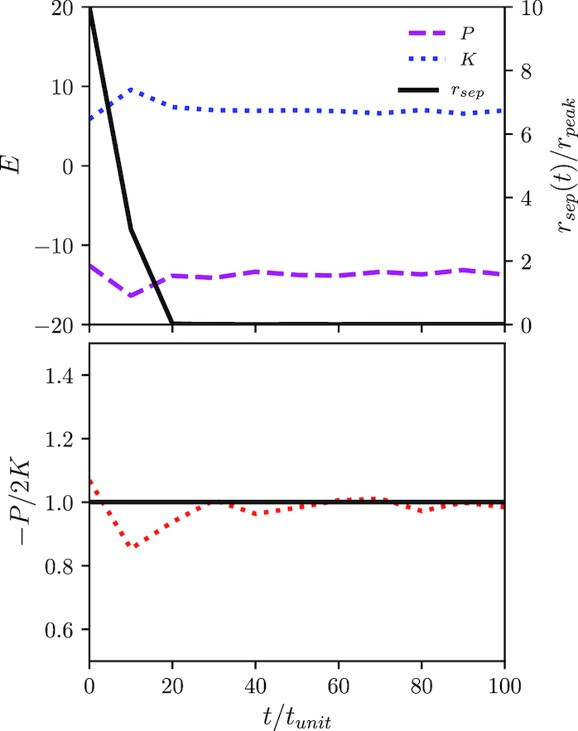
\includegraphics[width=.5\textwidth]{two_galaxy_merger.jpg}
\caption{Energy evolution of the system of two halos of same mass, merging together, as shown in \cite{same_mass_merger_1}. The progenitor galaxies possessed the Einasto density profiles. As can be seen in the bottom panel, after the merger, virial ratio (dotted red line) of the merger halo is nearly equal to 1.\label{fig:virial}}
\end{figure}

 We currently have an understanding of the energy evolution of the halos in a system of two galaxies as they merge \citep[e.g.][]{same_mass_merger_1, same_mass_merger_2}. The virial ratio of a galaxy is defined as, $- \frac{P}{2K}$, where $P$ is the total internal potential energy and $K$ is the total kinetic energy \citep{same_mass_merger_1}. When the virial ratio equals to 1, the galaxy is in virial equilibrium and is purely supported by velocity dispersion. Fig. \ref{fig:virial}, taken from \cite{same_mass_merger_1}, shows the merger remnant of two equal mass galaxies that is dominantly supported by velocity dispersion.

For a system of two galaxies, the total energy remains conserved as they merge into a single remnant as is obvious in the case of the simulation of two-galaxy system \citep{same_mass_merger_1}. However, we do not yet have a sound understanding of how the energy evolves in a more complex system containing more than two galaxies, which is the case in most galaxy mergers. As the given simulation contains a three-galaxy system, it is possible that the total energy of the MW and M31 may not remain conserved as there may be energy loss or gain from their interaction with M33. Understanding this interaction will help us understand the open problem of understanding galaxy mergers in systems with multiple galaxies. Furthermore, It is known that known halo shapes are mostly supported dominantly by anisotropic velocity dispersion as they rotate very slowly \citep{spin_param_explain}. However, do the major merger remnants like Samyog also follow this theory? It is also unknown how the structure of small satellite galaxies change as the major merger occurs in galaxy clusters. Finding answers to these open questions is essential to further our understand the galaxy evolution through mergers occurring within complex systems like our local group.

\section{This Project}
\label{sec:proj}
In this paper, we propose to investigate whether the halo of major merger remnant Samyog is supported by rotation or velocity dispersion by looking at its virial ratio. We will also look at the energy budgets of M33 as it evolves over time. For these purposes, we want to understand the distribution of internal and orbital energies between the three halos before the merger and compare them to the final distribution of internal and orbital energies between the halos of Samyog and M33. 

This project addresses both the open questions mentioned in Section \ref{sec:intro}. We will find out whether the halo of Samyog is dominantly dispersion supported or dominantly rotation supported. We will also investigate whether the halo of M33 gains energy or looses energy and how that changes its internal structure in terms of it being more dispersion depended or more rotation depended as the merger takes place.

The information of whether the galaxy halo is dispersion supported or rotation supported corresponds to the internal structure, density profile, and shape of the galaxy \citep{same_mass_merger_1, same_mass_merger_2}. Thus, answering the proposed questions is something very important in understanding galaxy evolution through a major merger. This project addresses these questions by looking at the different energy budgets of all the separate halos at a given time. Using those energy budgets, we can find the virial ratios for all the halos, which is the direct indicator of whether the halo is dominantly supported by dispersion or not.   

%We will do this by finding a dimensionless spin parameter that is further discussed in Section \ref{sec:prop}.

\section{Methodology}
\label{sec:method}

Based on the current observational data, the future interactions between MW and M31 galaxies have been studied broadly. One such study was carried out using a combination of collisionless N-body simulations and semi-analytic orbit integrations for the three-galaxy system of MW, M31, and M33 in \cite{simulation}. Here, the N-body simulation means a dynamical simulation of system of many particles governed by gravitational force.

To answer these questions, we will calculate the internal energies of the various halos according to the flowchart as shown in Fig. \ref{fig:flowchart}. We will first calculate the internal energies of MW, M31, and M33 at given times before the merger occurs, i.e. at $t < 5.86$ Gyr \citep[see][]{simulation}. After the merger, we will calculate the internal energies of Samyog and M33 at given times. We then calculate the virial ratios of Samyog's halo, at given times to see how it evolves after its formation. We will compare the virial ratios of MW and M33 at $t=0$ Gyr with Samyog's virial ratio evolution to understand the halo structure of a galaxy major merger compared to its progenitors. Finally, we will look at the evolution of M33's virial ratio throughout the merger process to understand merger's impact on the satellite galaxy.  

\begin{figure}[htbp]
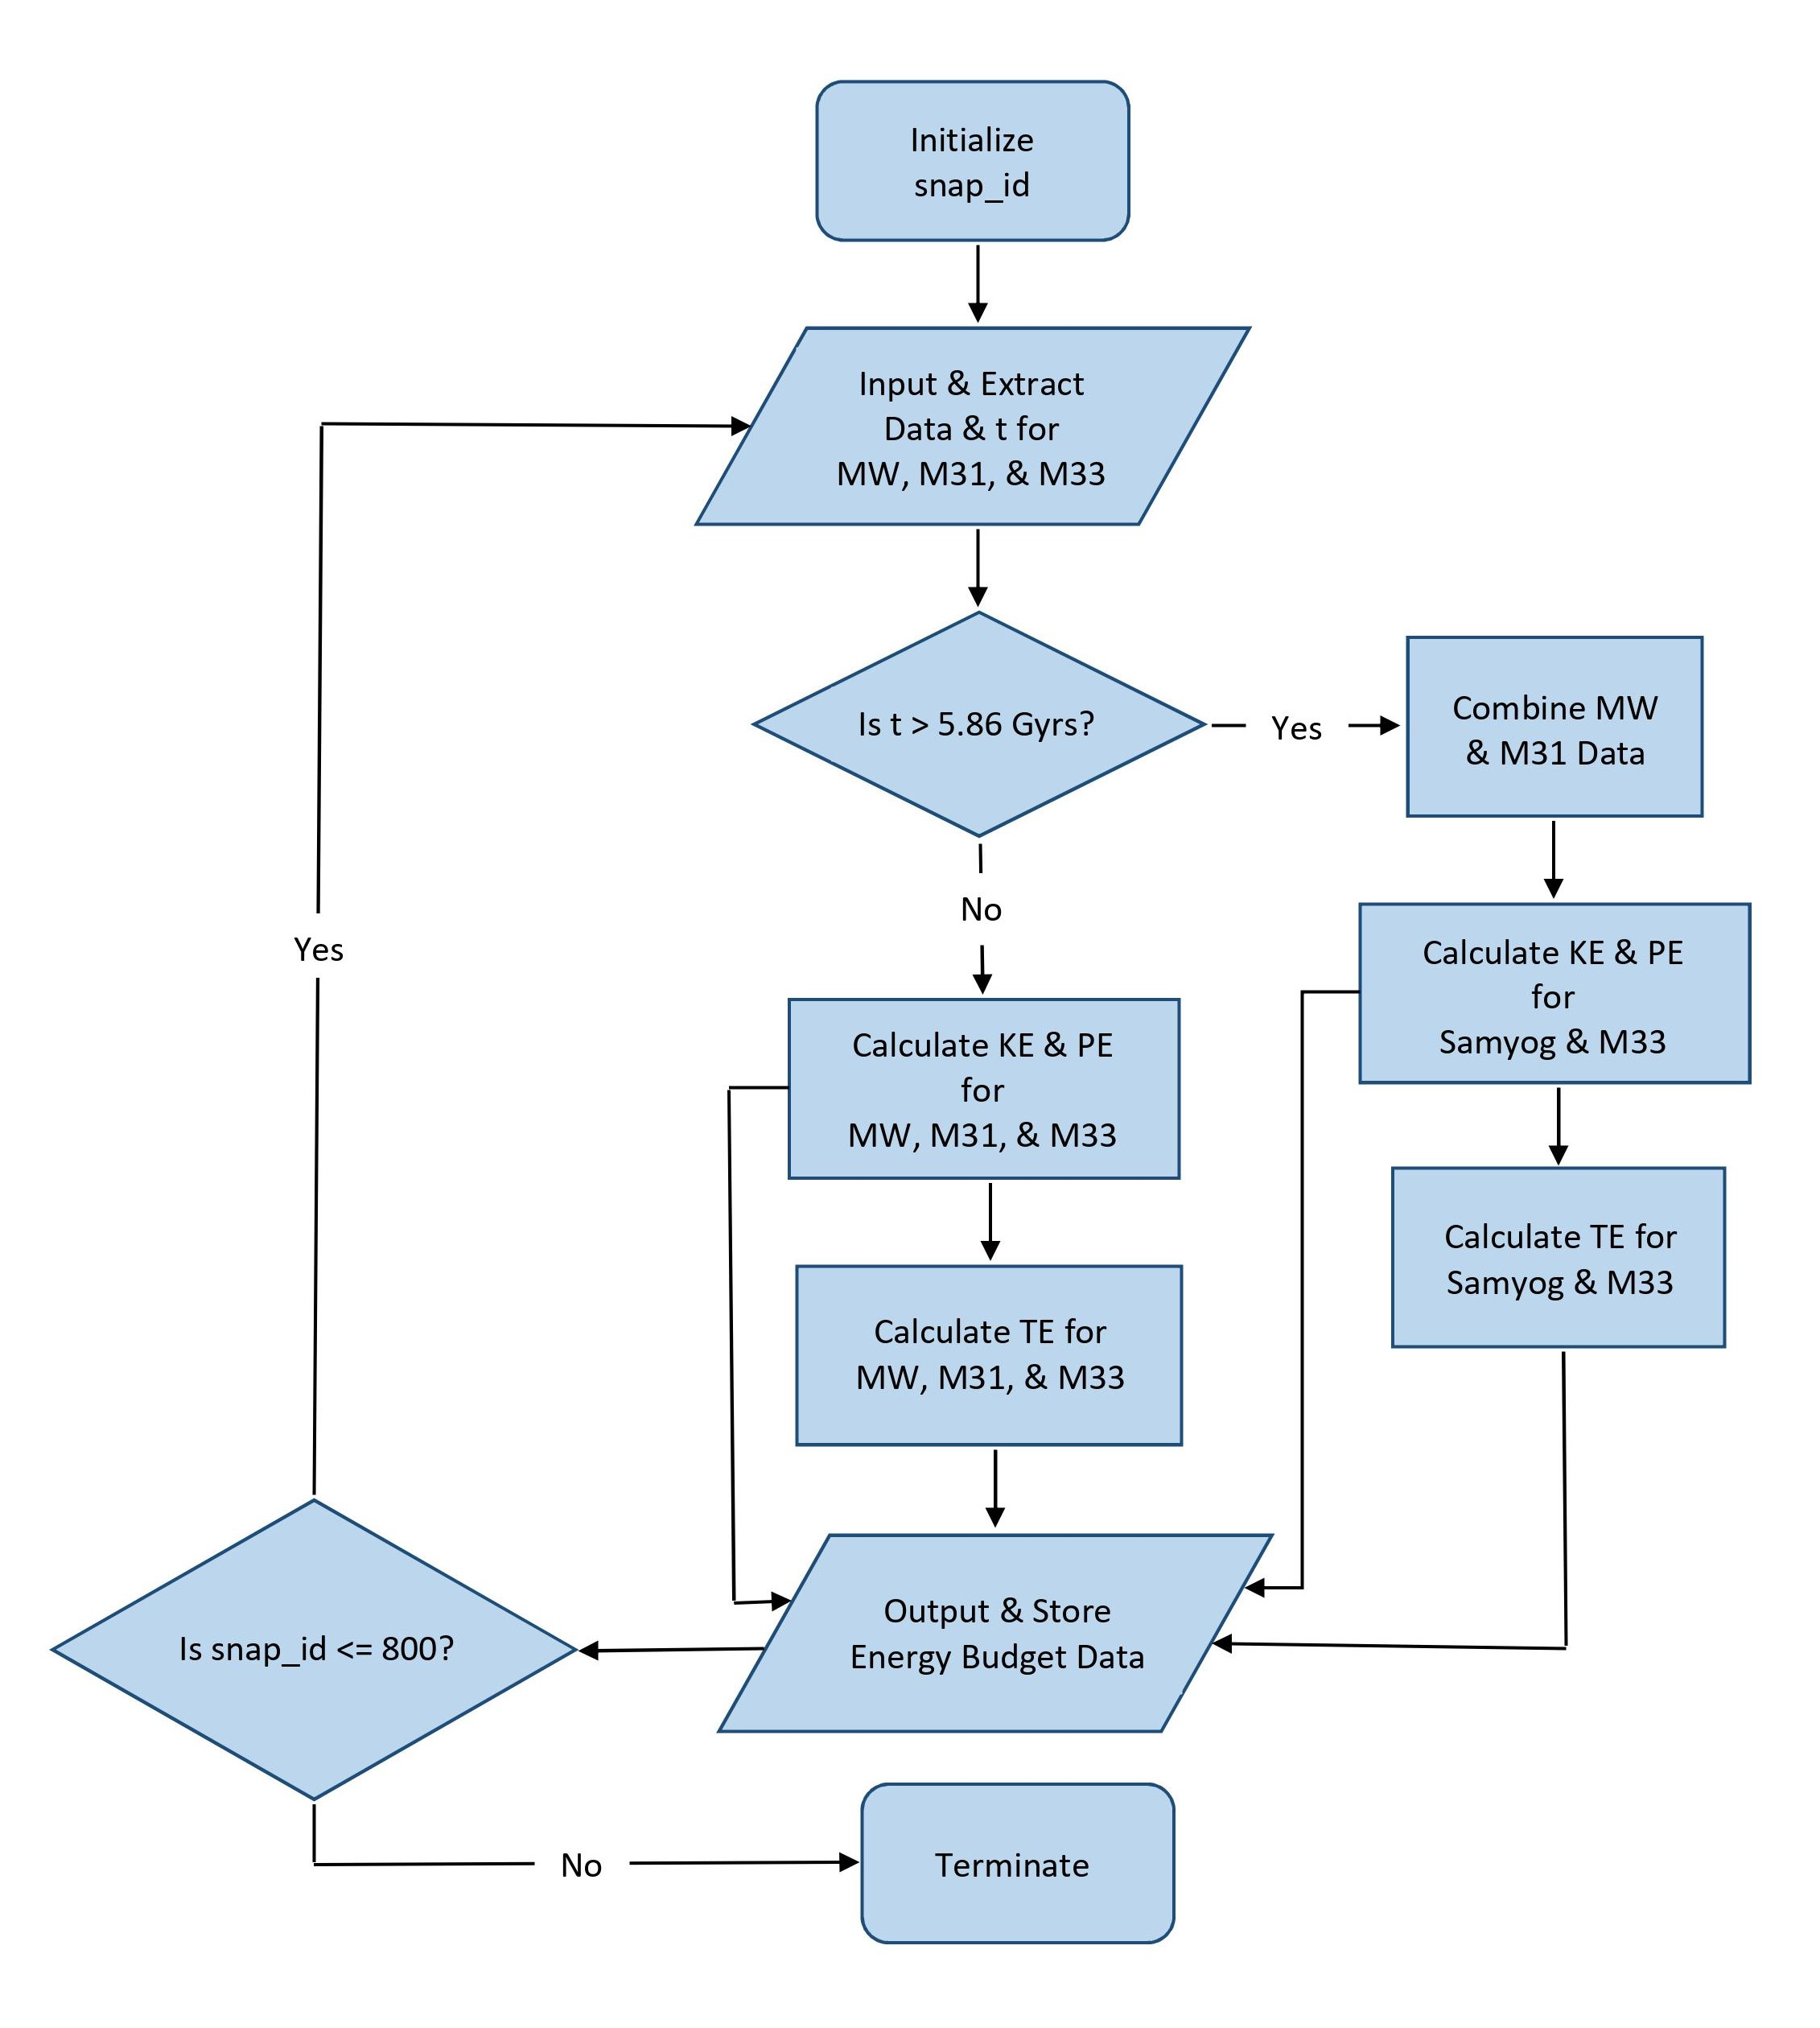
\includegraphics[width=.5\textwidth]{flowchart.jpg}
\caption{Flowchart showing the process of calculating internal energy budgets of different halos evolving with time. Note that the MW & M31 data is combined to calculate energy budgets of the halo of Samyog after time $t > 5.86$ Gyr, according to \cite{simulation}. 
\label{fig:flowchart}}
\end{figure}

We will investigate the total internal energies of the three galaxies before the merger occurs. This is done by using the equation for internal energy of the particular galaxy,
\begin{align}
    E_{int,g} = K_{int,g} + P_{int,g},
    \label{eq:internal_energy}
\end{align}
where $K_{int,g}$ is the kinetic energy of the halo and $P_{int,g}$ is the potential energy of the halo. These can be found using,
\begin{align}
    K_{int,g} &=\frac{1}{2}\Sigma_{i=1}^N m_i v_i^2, \nonumber \\ 
    P_{int,g} &= -\frac{1}{2} \Sigma_{i,j=1}^{N} \frac{G m_i m_j}{r_{ij}},
    \label{eq:kinetic_and_potential_energy}
\end{align}
where $N$ is the total number of particles in the given galaxy, $m_i$s are the masses of individual dark matter particles, $v_i$s are their speeds, and $r_{i,j}$s are the separations between the given two dark matter particles. If time allows, we will investigate various orbital energies to get an estimate of them. By comparing the loss of orbital energies to the internal energies gained by Samyog and M33 afte the merger will allow us to understand where the energy went during the merger and how it evolves the structures of the two halos. To find the orbital energies between any two galaxies, we will find the total energy between those two galaxies and subtract the internal energies of these galaxies,
\begin{align}
    E_{orb,g1-g2} = E_{tot,g1+g2} - E_{int,g1} - E_{int_g2}, \nonumber
\end{align}
which reduces to,
\begin{align}
    E_{orb,g1-g2} = -\frac{1}{2} \Sigma_{i=1}^{N_{g1}} \Sigma_{j=1}^{N_{g2}} \frac{G m_i m_j}{r_{ij}},
    \label{eq:orbital_energy}
\end{align}
where $N_{g1}$ and $N_{g2}$ are the total number of particles in the respective galaxies.

We will be plotting two figures as part of our results. The first figure will contain the virial ratio plots, similar to Fig. \ref{fig:virial}, of MW and M31 before the merger and of Samyog after the merger. The second figure will contain a single virial ratio plot of M33 over the entirety of the simulation time. These plots will be tremendous help in understanding the energy budget evolution of bot Samyog and M33. If time allows, we will plot the energy budgets of various orbital energies before and after the merger, which will help us understand the loss of total orbital energy as the time evolves.

We hypothesise that we will find that Samyog is nearer to virial equilibrium compared to the initial conditions of MW and M31. It is understandable that the major merger remnant, Samyog, will be `hotter' than either MW or M31 at $t=0$ Gyr. This means that the motion of dark matter particles within the halo is more random, giving us a virial ratio for the halo of Samyog to be nearer to 1. Thus, Samyog would be dominantly supported by velocity dispersion. We also hypothesize that M33 will also gain energy and become more random as it is loosing its orbital energy due to dynamical friction. 


%For the purpose of understanding the energy evolution of the system, we will investigate where the orbital potential energy being lost between the two galaxies go as they merge. We will do so by finding whether the change in rotation or velocity desperation of the Samyog is enough to account for this energy loss. We will also inquire whether Samyog is dominantly supported by rotation or by velocity dispersion. 

%Now, to calculate the total energy of the system, we will use the equation,
%\begin{align}
%    E_{tot} = \Sigma_{g} \, E_{int,g} + \Sigma_{g1 \neq g2} \, E_{orb,g1-g2}.
%    \label{eq:total_energy}
%\end{align} 

%Finally, to find the angular momentum of the halo, we use the equation,
%\begin{align}
%    \bold{J} = \Sigma_{i=1}^{N} m_i \bold{r_i} \times \bold{v_i}.
%    \label{eq:angular_momentum}
%\end{align}

%To understand whether the halo is dominantly supported by rotation or velocity dispersion, a dimensionless spin parameter, $\lambda$, can be useful. The spin parameter is defined as,
%\begin{align}
%    \lambda = \frac{J |E|^{1/2}}{G M^{5/2}},
%    \label{eq:spin_param}
%\end{align}
%where $M$ is the halo mass, $J$ is the magnitude of its angular momentum, and $E$ is the internal energy of the halo \citep{spin_param_explain, same_mass_merger_1}. 
%According to \cite{spin_param_explain}, for a purely rotationally supported halo, $\lambda = 0.4$. As shown here in Fig. \ref{fig:spin_vs_energy}, taken from \cite{same_mass_merger_1}, the value of $\lambda$ of a merger can vary greatly depending on the initial conditions of its progenitors. However as stated before, it is known that halo shapes are mostly supported dominantly by anisotropic velocity dispersion as they rotate very slowly \citep{spin_param_explain}. Thus, using this parameter, we will be able to understand whether the remnant, Samyog, is supported by rotation or velocity dispersion. Depending on whether M33 gains or loses internal energy after the merger, we will also look at its spin parameter to understand the evolution of its spin parameter as the MW and M31 merges. We will look at the total internal energy of the M33 as well as the orbital energy in between M33 and Samyog to see whether the loss or gain of energy results into change in the internal structure of the M33 or does it only result in getting M33 to be gravitationally bound more or less to the remnant.    

%\begin{figure}[htbp]
%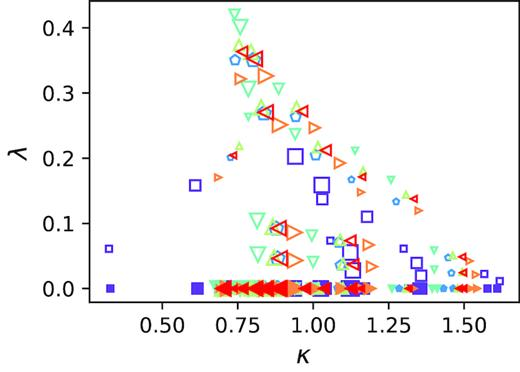
\includegraphics[width=.5\textwidth]{rotation_vs_dispersion.jpeg}
%\caption{The plot of spin parameter vs energy parameter for various galaxy merger remnants according to different initial conditions as shown in \cite{same_mass_merger_1}. As can be seen in the plot there are a couple of merger remnants that are quite close to $\lambda=0.4$, attributing to them being purely supported by rotation. The value of $\lambda$ is very spread out giving us the understanding that the merger remnants can be dominantly supported by rotation, which is in contrast to the statement given in \cite{spin_param_explain}, given that they have some particular initial conditions. \label{fig:spin_vs_energy}}
%\end{figure}

%To find these values from our N-body simulation, we will first write a code to find the Center Of Mass of the MW at t=0. We will use this point as the point of origin for all the following calculations using the simulation data. Thus, whenever we read the data from any of the snapshot, we will convert the data to the reference frame of this CoM of the MW at $t=0$ Gyr. 

%Then, we will write the codes for finding the internal kinetic energy and the internal potential energy for any galaxy using eq. \ref{eq:kinetic_and_potential_energy}. We will write the code to calculate the total internal energy by utilizing eq. \ref{eq:internal_energy}.
%We will also implement the code to find the orbital energy between the two galaxies using eq. \ref{eq:orbital_energy}. Then, we will write the code to find the total energy of the system using eq. \ref{eq:total_energy}. We will implement the code to calculate the angular momentum of any given galaxy using eq. \ref{eq:angular_momentum}. Finally, we will implement the code to find the spin parameter of any given galaxy using eq. \ref{eq:spin_param}.  

%Since, we are interested in comparing the outcomes before and after the merger, we will take on the snapshots 0 and 800, corresponding to $t=0$ Gyr and $t~12$ Gyr, respectively. Using the 0th snapshot, we will find the internal energies, angular momentum, and spin parameters of all three galaxies. We will also find the orbital energies of the galaxy pairs and then find the the total energy of the system. We will also find the total energy of the MW and M31 system by adding up both of their internal energies with the orbital energy between them. Then, using the 800th snapshot, we will find the internal energies, angular momentum, and spin parameters of both the galaxies, Samyog and M33. We will also find the orbital energy and total energy of this system. Finally, we will compare the internal energy of Samyog at snapshot 800 to the total energy of the MW and M31 system found at snapshot 0 to fins the answer to our first question. Then, we will look at the spin parameters of Samyog to understand whether it is dominantly supported by rotation or velocity dispersion. Finally, we will look at the spin parameter and internal energy of M33 along with the orbital energy of the Samyog-M33 system to understand how the merger has impacted M33.   

%-------------

\bibliography{bibs}{}
\bibliographystyle{aasjournal}

\end{document}

